\section{Reservoir Computing}

\begin{frame}{Reservoir computing}

	\begin{itemize}
		\item Special kind of artificial neural network
		\item State of the art performances for:
		\begin{itemize}
			\item Real-time data processing
			\item Chaotic time series prediction
			\item Speech-recognition
			\item Nonlinear communication channel equalisation
			\item Financial forecasting
		\end{itemize}
		\item Machine learning computationally lighter than the majority of artificial neural networks
		\item Scheme imposes very few constraints \\$\Longrightarrow$ implementation in physical systems possible !
	\end{itemize}

\end{frame}

\begin{frame}{Mathematical model}

	\begin{columns}
		\begin{column}{.5\textwidth}
			\begin{figure}
				\centering
				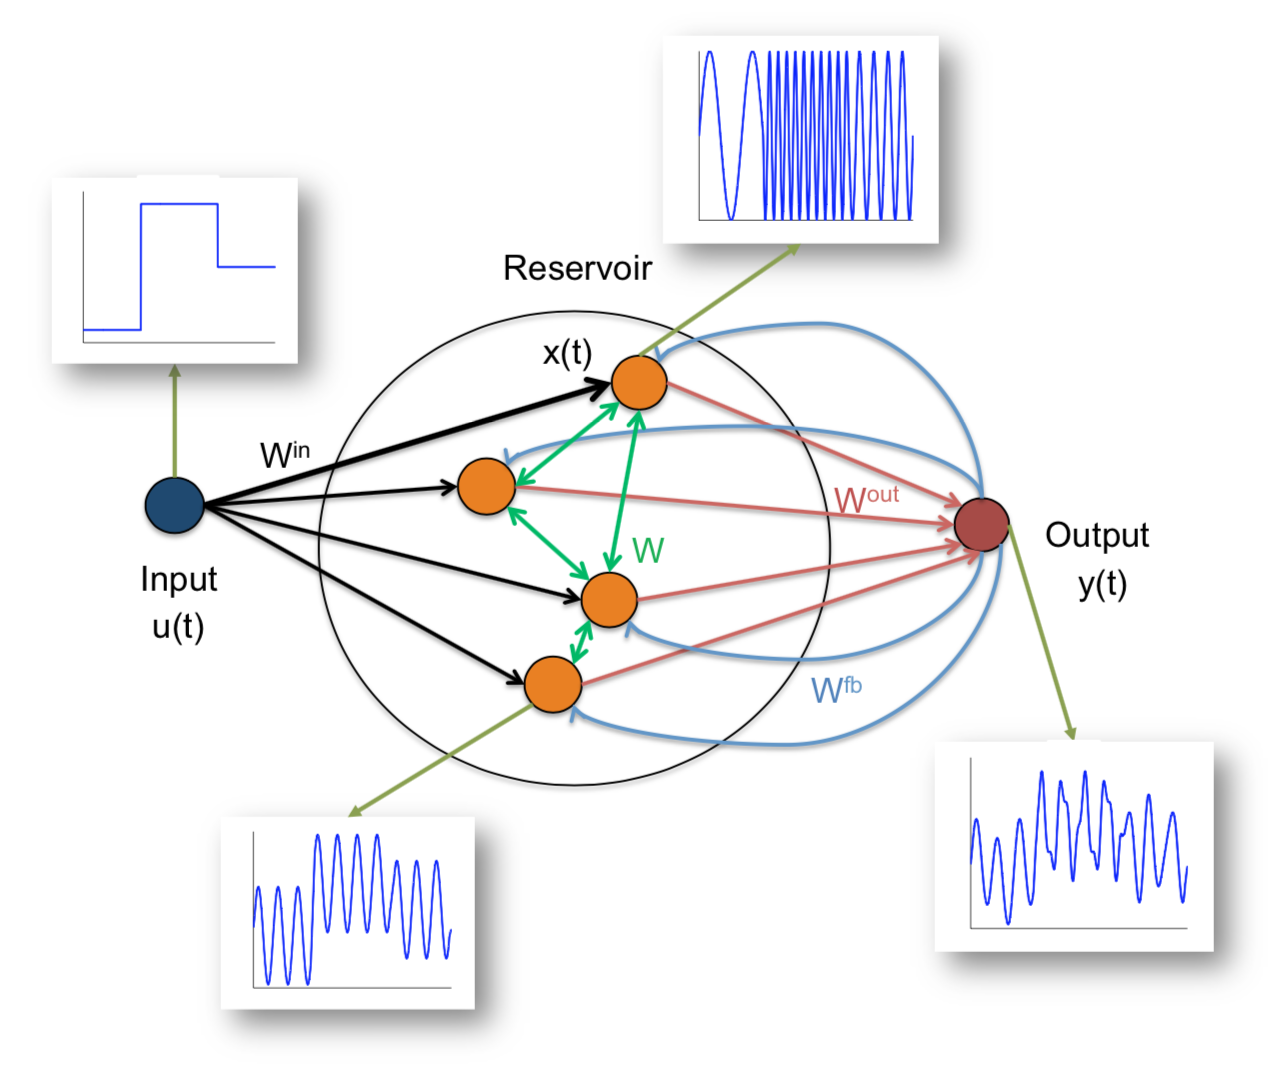
\includegraphics[width=\textwidth]{rc_principle.png}
				\caption{\cite{financialTimeSeries}}
			\end{figure}
		\end{column}%
		\begin{column}{.5\textwidth}
			\begin{itemize}
				\item $\mathbf{x}$ : state vector (activation levels of the neurons)
				\item $u$ : input signal
				\item $y$ : output signal
				\item $\mathbf{W}^{\text{in}}$ : input matrix
				\item $\mathbf{W}$ : connection matrix
				\item $\mathbf{W}^{\text{out}}$ : output matrix
			\end{itemize}
			\begin{alertblock}{}
				\begin{align}
				\mathbf{x}(n+1) &= \mathbf{f} \left( \mathbf{W}^{\text{in}} u(n+1) + \mathbf{W} \mathbf{x}(n) \right) \nonumber \\
				y(n+1) &= f^{\text{out}}\left( \mathbf{W}^{\text{out}} \mathbf{x}(n+1) \right) \nonumber
			\end{align}
			\end{alertblock}
		\end{column}
	\end{columns}

\end{frame}

\begin{frame}{Photonic reservoir computing}
	\begin{columns}
		\begin{column}{.5\textwidth}
			\begin{figure}
				\centering
				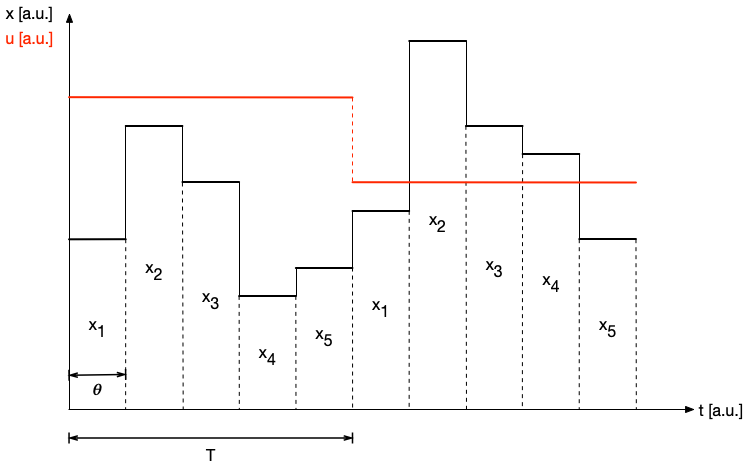
\includegraphics[width=\textwidth]{tdm-neurons-principle.png}
			\end{figure}
		\end{column}%
		\begin{column}{.5\textwidth}
			\begin{itemize}
				\item So far in optical systems, only \textbf{Time Division Multiplexing} of the neurons
				\item Two main families of optical encoding of the neurons:
				\begin{itemize}
					\item In the phaser of the electric field : $x_i = E_i$
					\item In the intensity of the light : $x_i = |E_i|^2$
				\end{itemize}
			\end{itemize}
		\end{column}
	\end{columns}
\end{frame}

\begin{frame}{Numerical simulations - NARMA10}
	\begin{figure}
		\centering
		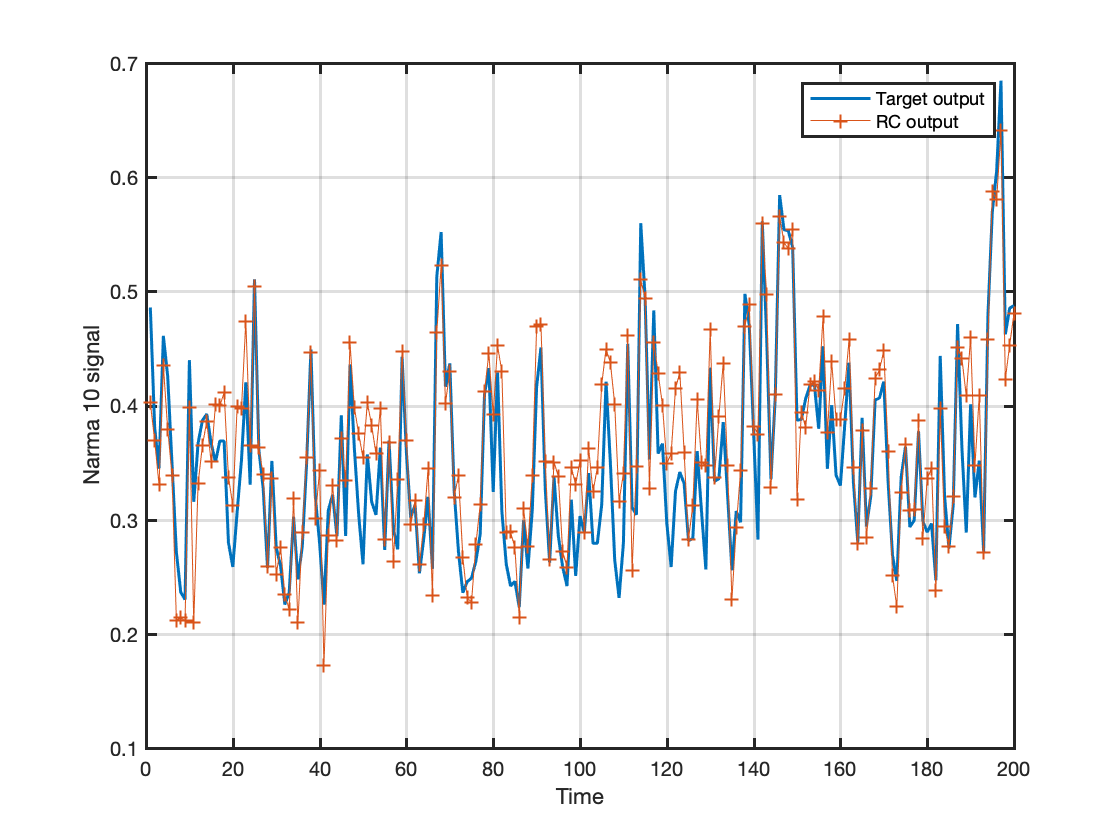
\includegraphics[width=.9\textwidth]{narma10.png}
		\caption{Simulation with 50 neurons. Normalised Mean Square Error of 0.1541.}
	\end{figure}
\end{frame}

\begin{frame}{Numerical simulations - nonlinear channel equalisation}
	\begin{figure}
		\centering
		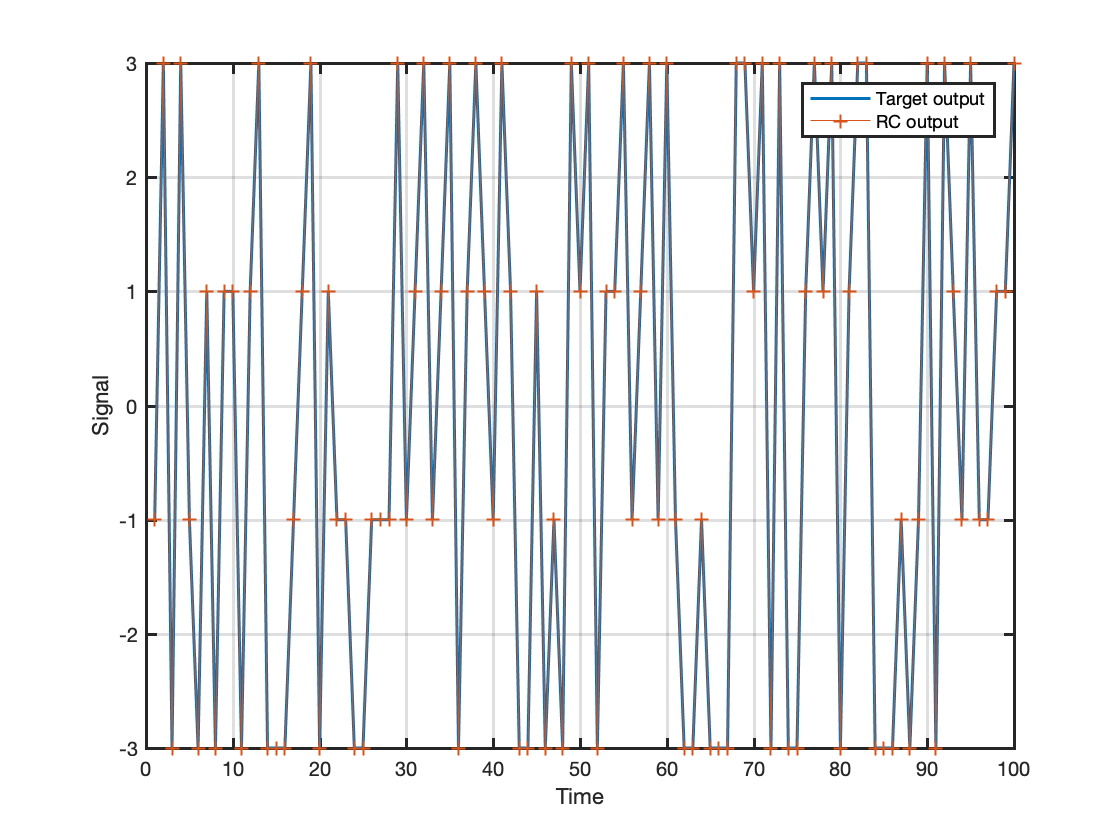
\includegraphics[width=.85\textwidth]{nonlinear_ch_eq.png}
		\caption{Simulation with 50 neurons. Signal-to-Noise Ratio of \SI{32}{\dB}. Signal Error Rate of \num{5e-4}.}
	\end{figure}
\end{frame}